\Problem
{گام اول}
{
    با توجه به حجم زیاد نرم‌افزار متلب و کمبود فضا، از نرم‌افزار 
    \lr{GNU Octave} 
    استفاده کردم که دارای دو محیط کاربری متنی و گرافیکی است.
    
    این برنامه تمامی دستورات متلب را پشتیبانی می‌کند و قابلیت بارگذاری پکیج‌ها و تولباکس‌های متلب را دارد. 
    
    برای مثال با دستور زیر می‌توانیم پکیج مربوط بهه انتقال داده متلب را بارگذاری کنیم:
    
    \lr{\LTR{pkg load communications}}
    
    \begin{figure}[H]
        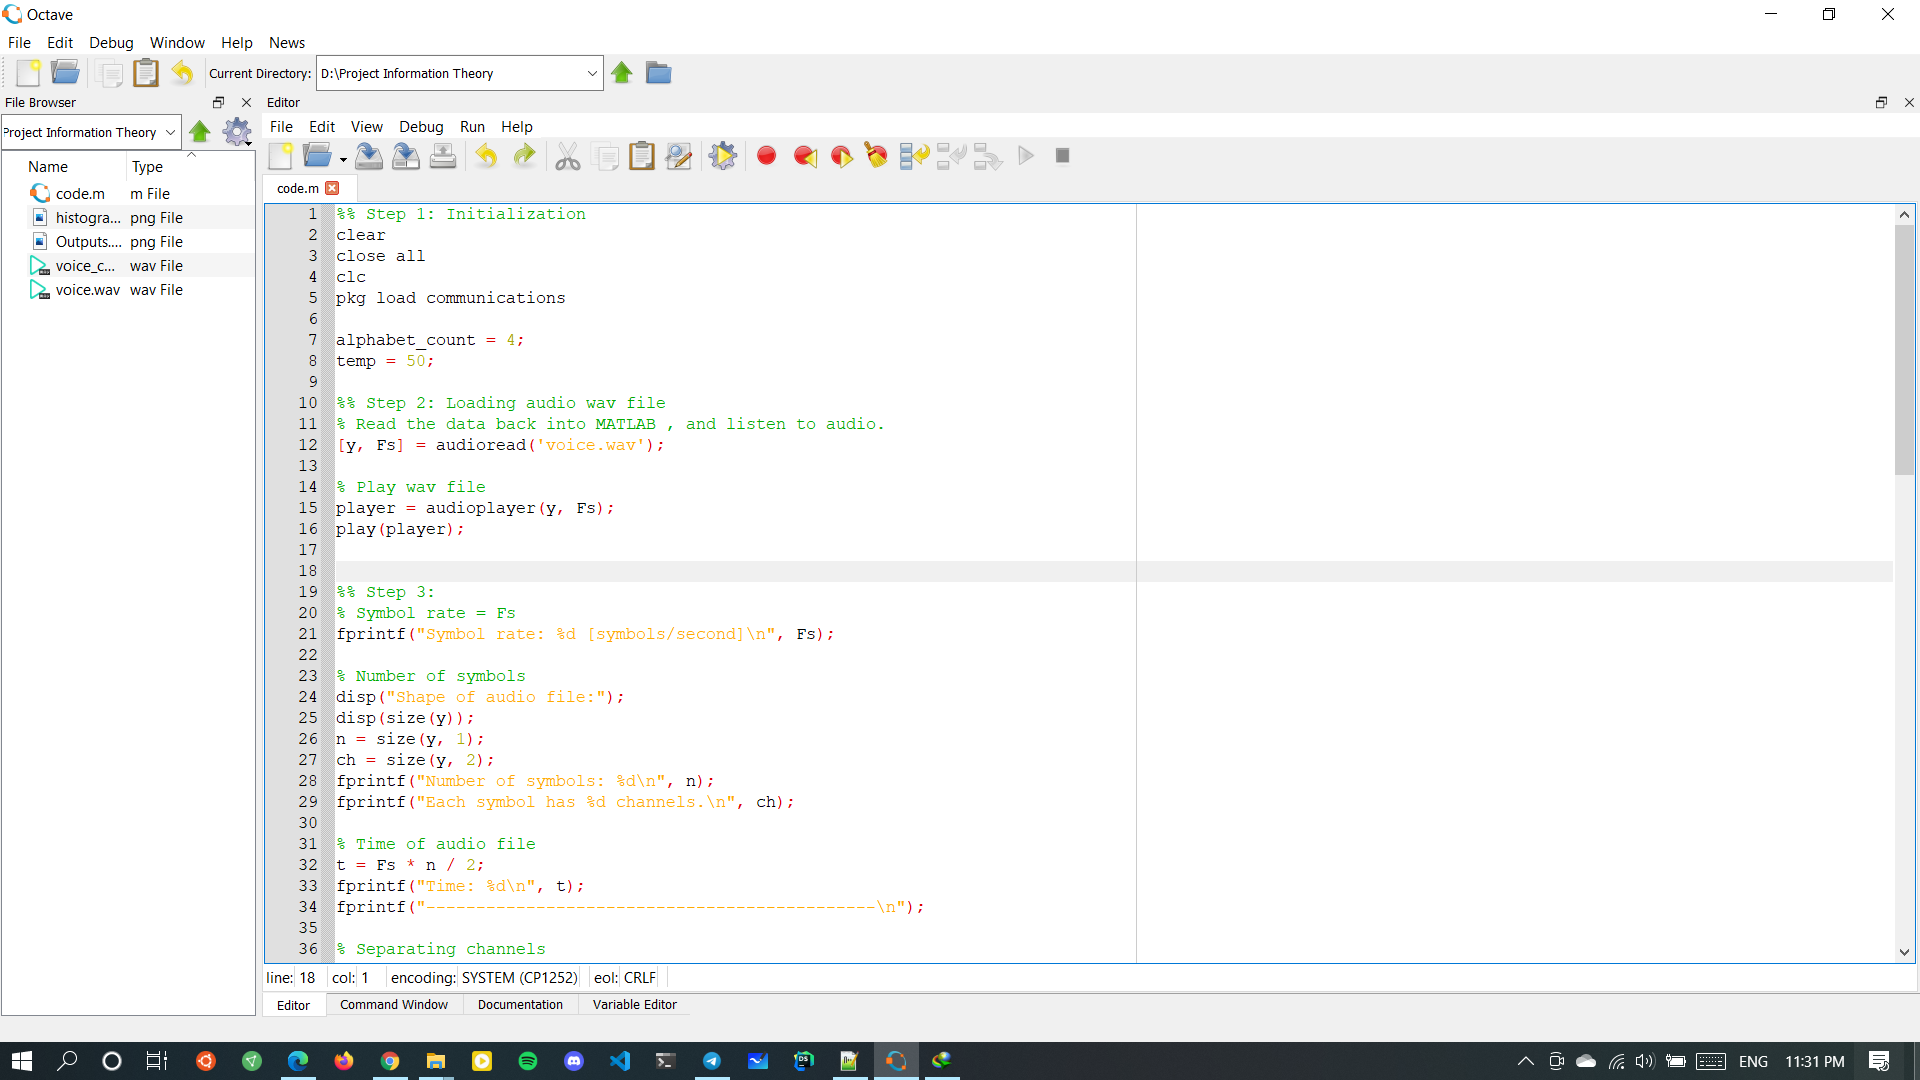
\includegraphics[width=15cm]{Images/Octave.png}
        \centering
        \caption{محیط \lr{Octave}}
    \end{figure}
}
